% ICD Sketch Diagram for SCS Protocol
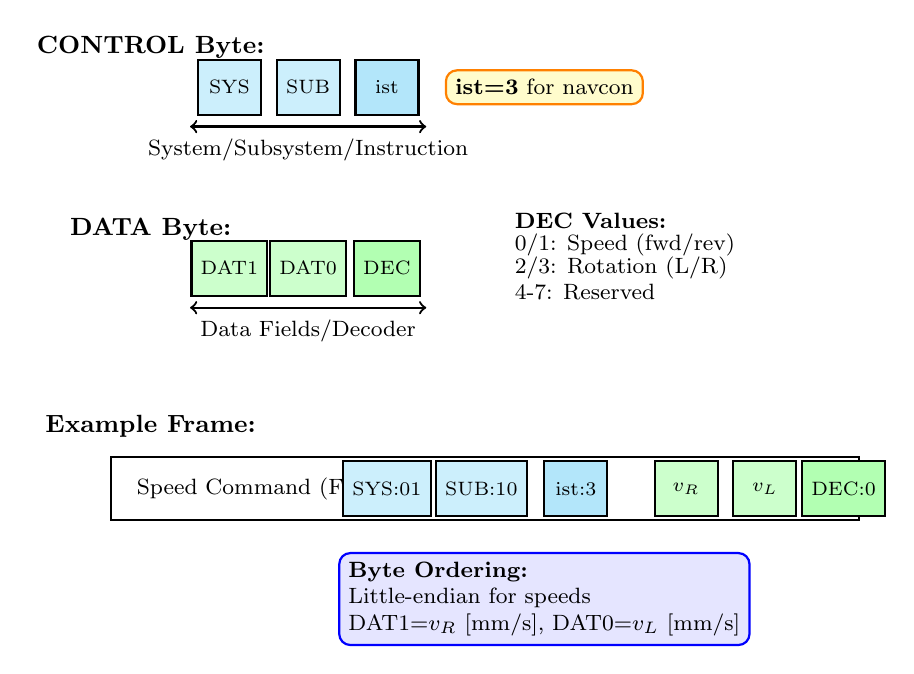
\begin{tikzpicture}[
  bitbox/.style={rectangle, draw=black, thick, minimum width=0.8cm, minimum height=0.7cm, font=\scriptsize},
  label/.style={font=\small\bfseries},
  description/.style={font=\footnotesize}
]

% CONTROL Byte
\node[label] at (0, 3.5) {CONTROL Byte:};

\node[bitbox, fill=cyan!20] (sys) at (1, 3) {SYS};
\node[bitbox, fill=cyan!20] (sub) at (2, 3) {SUB};
\node[bitbox, fill=cyan!30] (ist) at (3, 3) {\gls{ist}};

\draw[<->, thick] (0.5, 2.5) -- (3.5, 2.5);
\node[description] at (2, 2.2) {System/Subsystem/Instruction};

% IST=3 highlight
\node[description, fill=yellow!20, draw=orange, thick, rounded corners] at (5, 3) {\textbf{\gls{ist}=3} for \gls{navcon}};

% DATA Byte
\node[label] at (0, 1.2) {DATA Byte:};

\node[bitbox, fill=green!20] (dat1) at (1, 0.7) {DAT1};
\node[bitbox, fill=green!20] (dat0) at (2, 0.7) {DAT0};
\node[bitbox, fill=green!30] (dec) at (3, 0.7) {DEC};

\draw[<->, thick] (0.5, 0.2) -- (3.5, 0.2);
\node[description] at (2, -0.1) {Data Fields/Decoder};

% DEC Field Legend
\node[description, anchor=west] at (4.5, 1.3) {\textbf{DEC Values:}};
\node[description, anchor=west] at (4.5, 1.0) {0/1: Speed (fwd/rev)};
\node[description, anchor=west] at (4.5, 0.7) {2/3: Rotation (L/R)};
\node[description, anchor=west] at (4.5, 0.4) {4-7: Reserved};

% Example Frame
\node[label] at (0, -1.3) {Example Frame:};

\draw[thick, draw=black] (-0.5, -2.5) rectangle (9, -1.7);
\node[description, anchor=west] at (-0.3, -2.1) {Speed Command (Forward):};

\node[bitbox, fill=cyan!20] at (3, -2.1) {SYS:01};
\node[bitbox, fill=cyan!20] at (4.2, -2.1) {SUB:10};
\node[bitbox, fill=cyan!30] at (5.4, -2.1) {\gls{ist}:3};
\node[bitbox, fill=green!20] at (6.8, -2.1) {$v_R$};
\node[bitbox, fill=green!20] at (7.8, -2.1) {$v_L$};
\node[bitbox, fill=green!30] at (8.8, -2.1) {DEC:0};

% Byte ordering note
\node[description, fill=blue!10, draw=blue, thick, rounded corners, align=left] at (5, -3.5) {
  \textbf{Byte Ordering:}\\
  Little-endian for speeds\\
  DAT1=$v_R$ [mm/s], DAT0=$v_L$ [mm/s]
};

\end{tikzpicture}
